\documentclass[accentcolor=tud2c,usenames,dvipsnames,colorbacktitle,inverttitle,landscape,german,presentation,t]{tudbeamer}
\usepackage[english]{babel}
\usepackage{amsmath}
\usepackage{amssymb}
\usepackage{color}
\usepackage{graphicx}
\usepackage{braket}
\usepackage[utf8]{inputenc}

\begin{document}

\title{Shell evolution in nuclei}
\subtitle{\small{Matthias Heinz}}
\author{Matthias Heinz, advised by Prof.\ Dr.\ Alexandre Obertelli}
\institute[Institut f\"ur Kernphysik, TU Darmstadt]{Institut f\"ur Kernphysik, TU Darmstadt}
\date{December 20, 2018}

\setbeamertemplate{section in toc}[ball unnumbered]
\setbeamertemplate{subsection in toc}[ball unnumbered]

\nocite{*}

\begin{titleframe}
  \begin{center}
    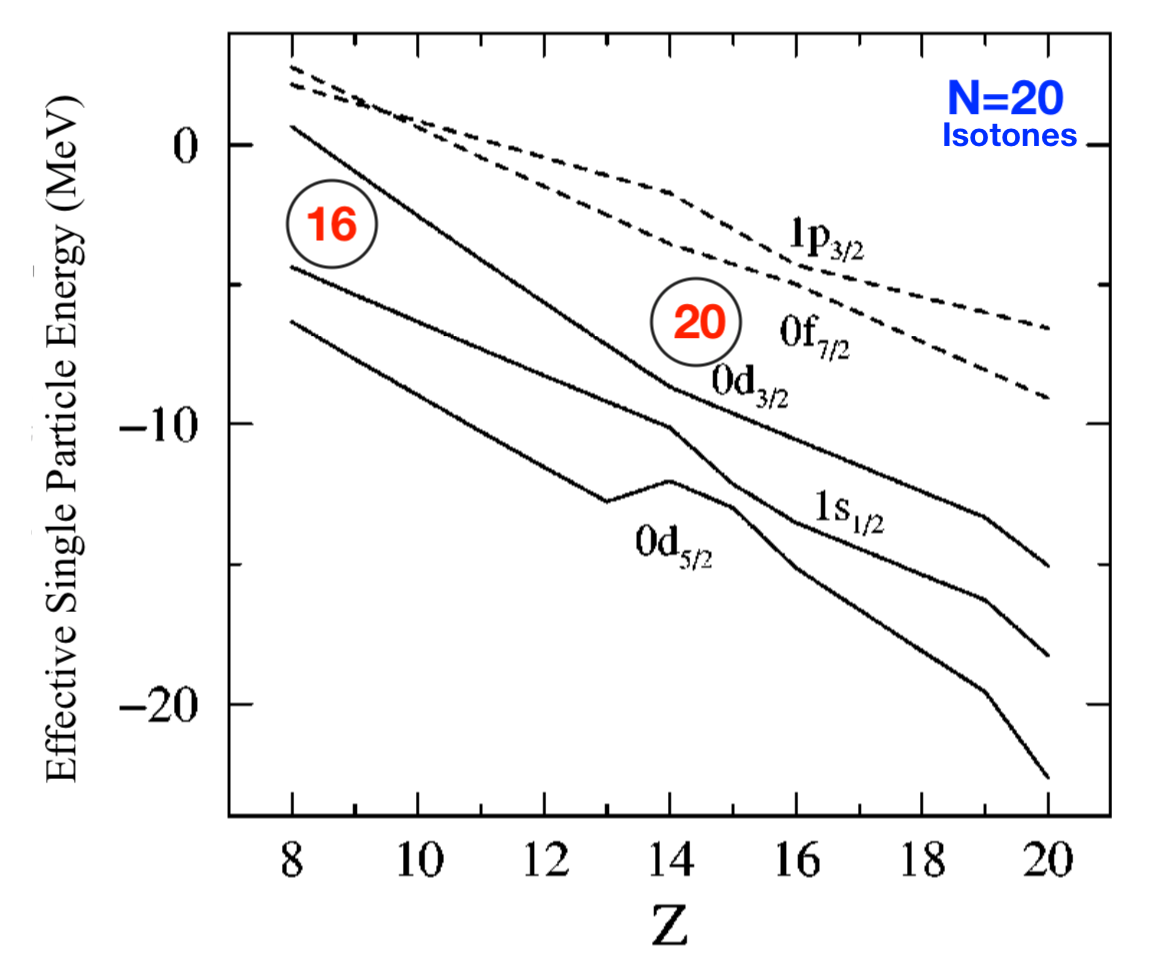
\includegraphics[trim={1.4cm 0 0 0},clip,width=0.55\textwidth]{images/utsuno_edited}
    \\ \small{\cite{Utsuno:1999st}}
  \end{center}
\end{titleframe}

\begin{frame}
  \frametitle{Outline}
  \tableofcontents
\end{frame}

\section{Overview of the Shell Model}

  \begin{frame}
    \frametitle{Nuclear Shell Model}
    \vskip-3em
    \begin{columns}[c]
      \begin{column}{0.5\textwidth}
        \begin{block}{}
          \begin{itemize}
            \item Mean field and NN correlations
            \item Valence space for ``active nucleons''
            \item Shell gaps and correlations (configuration mixing)
            \item Magic nuclei: closed shells for protons and/or neutrons
          \end{itemize}
        \end{block}
      \end{column}
      \begin{column}{0.5\textwidth}
        \begin{block}{}
          \begin{center}
            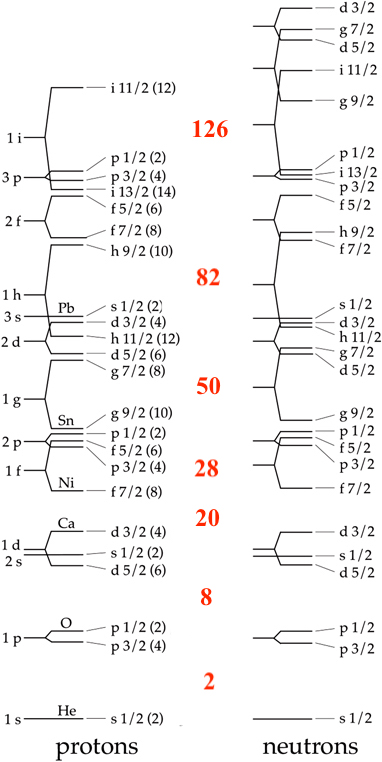
\includegraphics[trim={0 0 0 0.8cm},clip,width=0.48\textwidth]{images/shell_model}
            \\ \small{\cite{10.1088/978-0-7503-1140-3ch6}}
          \end{center}
        \end{block}
      \end{column}
    \end{columns}
  \end{frame}

  \begin{frame}
    \frametitle{Shell Evolution}
    \begin{itemize}
      \item Monopole drift
      \item Consider interaction between $p_{3/2}$ \textcolor{red}{protons} and the single \textcolor{blue}{neutron}
    \end{itemize}
    \begin{equation*}
      \color{black} \braket{\textcolor{red}{j^2} (J=0) \textcolor{blue}{j'}|V_{1n} + V_{2n}|\textcolor{red}{j^2} (J=0) \textcolor{blue}{j'}}
      = 2 \sum_{J=|j-j'|}^{j+j'} (2J+1)\braket{\textcolor{red}{j}\textcolor{blue}{j'}J|V|\textcolor{red}{j}\textcolor{blue}{j'}J}/\sum_{J=|j-j'|}^{j+j'} (2J+1)
    \end{equation*}
    \vskip-3em
    \begin{columns}[c]
      \begin{column}{0.5\textwidth}
        \begin{block}{}
          \begin{itemize}
            \item Spin and isospin dependence
            \item Monopole vs.\ multi-pole correlations
          \end{itemize}
        \end{block}
      \end{column}
      \begin{column}{0.5\textwidth}
        \begin{block}{}
          \begin{center}
            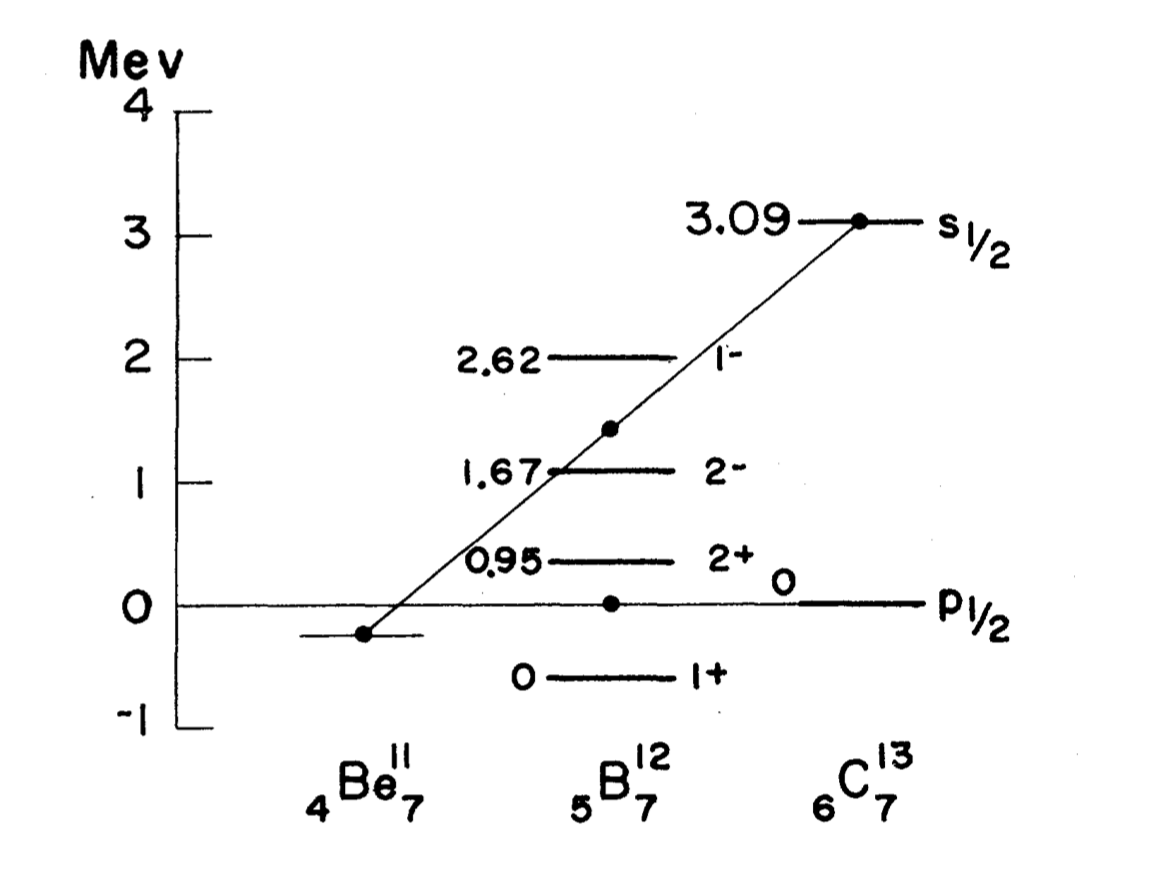
\includegraphics[trim={0 0 0 0.0cm},clip,width=0.7\textwidth]{images/talmi1}
            \\ \small{\cite{Talmi:1960zz}}
          \end{center}
        \end{block}
      \end{column}
    \end{columns}
  \end{frame}

  \begin{frame}
    \frametitle{Properties of ``Magic Nuclei''}
    \vskip-2em
    \begin{columns}[c]
      \begin{column}{0.4\textwidth}
        \begin{block}{}
          Properties of ``magic nuclei'':
          \begin{itemize}
            \item Large binding energy
            \item Long lifetime
            \item High excitation energy
            \item Low $B(E2)$
            \item Spherical $\rightarrow$ small $r_{rms}$
          \end{itemize}
        \end{block}
      \end{column}
      \begin{column}{0.6\textwidth}
        \begin{center}
          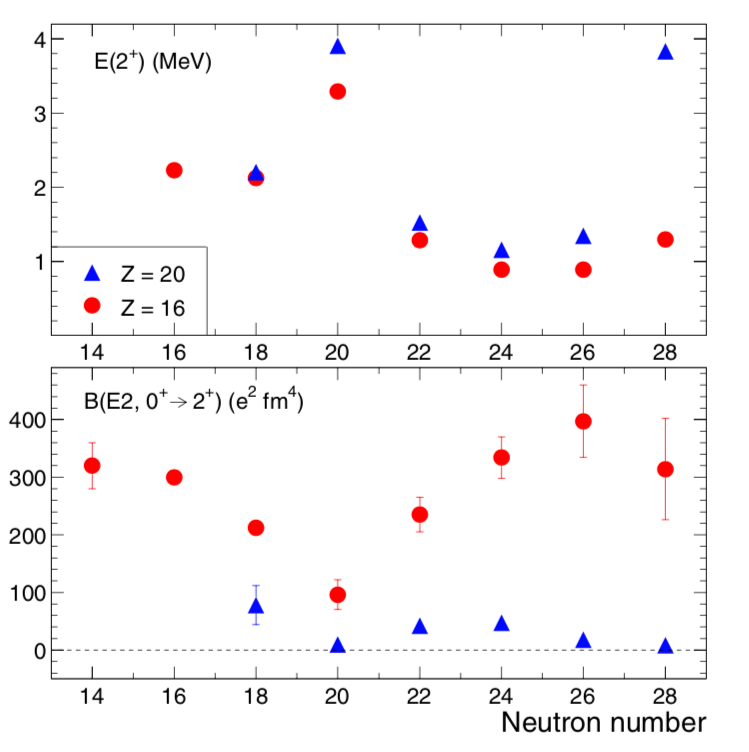
\includegraphics[width=0.85\textwidth]{images/alamanos}
          \\ \small{\cite{Alamanos:2004review}}
        \end{center}
      \end{column}
    \end{columns}
  \end{frame}

\section{Motivation}

  \begin{frame}
    \frametitle{Motivation}
    \vskip-3em
    \begin{columns}[t]
      \begin{column}{0.45\textwidth}
        \begin{block}{}
          Historical example:
          \begin{itemize}
            \item $N=20$ shell disappearance
            \item $N=16$ shell appearance
          \end{itemize}
        \end{block}
      \end{column}
      \begin{column}{0.55\textwidth}
        \begin{block}{}
          Experimental challenges:
          \begin{itemize}
            \item Large range of unstable, bound nuclei
            \item Beam intensity quickly drops to 0
          \end{itemize}
        \end{block}
      \end{column}
    \end{columns}
    \begin{center}
      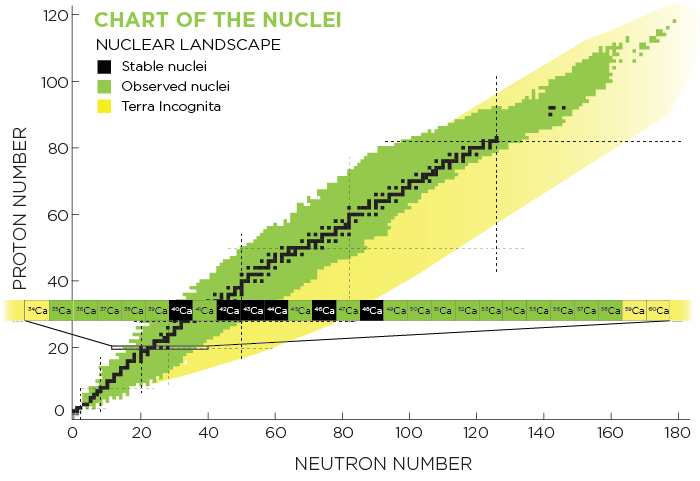
\includegraphics[width=0.47\textwidth]{images/nscl}
      \\ \small{\cite{Nscl:2018web}}
    \end{center}
  \end{frame}

\section{Disappearance of $N=20$ Shell Closure}

  \begin{frame}
    \frametitle{Observable: $B(E2)$}
    \begin{itemize}
      \item Reduced electric quadrupole transition probability
    \end{itemize}
    \begin{center}
      \begin{equation*}
        B(E2:J_i\rightarrow J_f)=\frac{1}{2J_i + 1} | \braket{\psi_f | E2 | \psi_i} |^2
      \end{equation*}
    \end{center}
    \begin{itemize}
      \item Measured via intermediate Coulomb excitation
      \begin{itemize}
        \item Required intensity: \textasciitilde100 pps
        \item Precision: \textasciitilde10--15\%
      \end{itemize}
      \item Alternative: low-energy Coulomb excitation
       \begin{itemize}
        \item Required intensity: several thousand pps
      \end{itemize}
      \item Alternative: lifetime measurement
      \begin{itemize}
        \item Required intensity: several thousand pps
      \end{itemize}
    \end{itemize}
  \end{frame}

  \begin{frame}
    \frametitle{Coulomb Excitation of $^{32}Mg$ \\ \small{\textit{Motobayashi et al.}}}
    \vskip-2em
    \begin{columns}[c]
      \begin{column}{0.55\textwidth}
        \begin{block}{}
          \begin{itemize}
            \item $^{32}Mg$ beam on $^{208}Pb$ target
            \item Beam energy $49.2$ MeV/u
            \item Measure only forward angles
            \item Extract $B(E2)$ from cross section
          \end{itemize}
          \begin{equation*}
            \sigma_{E2} \approx {(\frac{Z e^2}{\hslash c})}^2 \frac{\pi}{e^2 b_{\min}^2} B(E2)
          \end{equation*}
          \begin{itemize}
            \item $\sigma=91.7\pm14.4$ mb
            \item $B(E2)=454\pm 78$ e\textsuperscript{2}fm\textsuperscript{4}
          \end{itemize}
        \end{block}
      \end{column}
      \begin{column}{0.45\textwidth}
        \begin{block}{}
          \begin{center}
            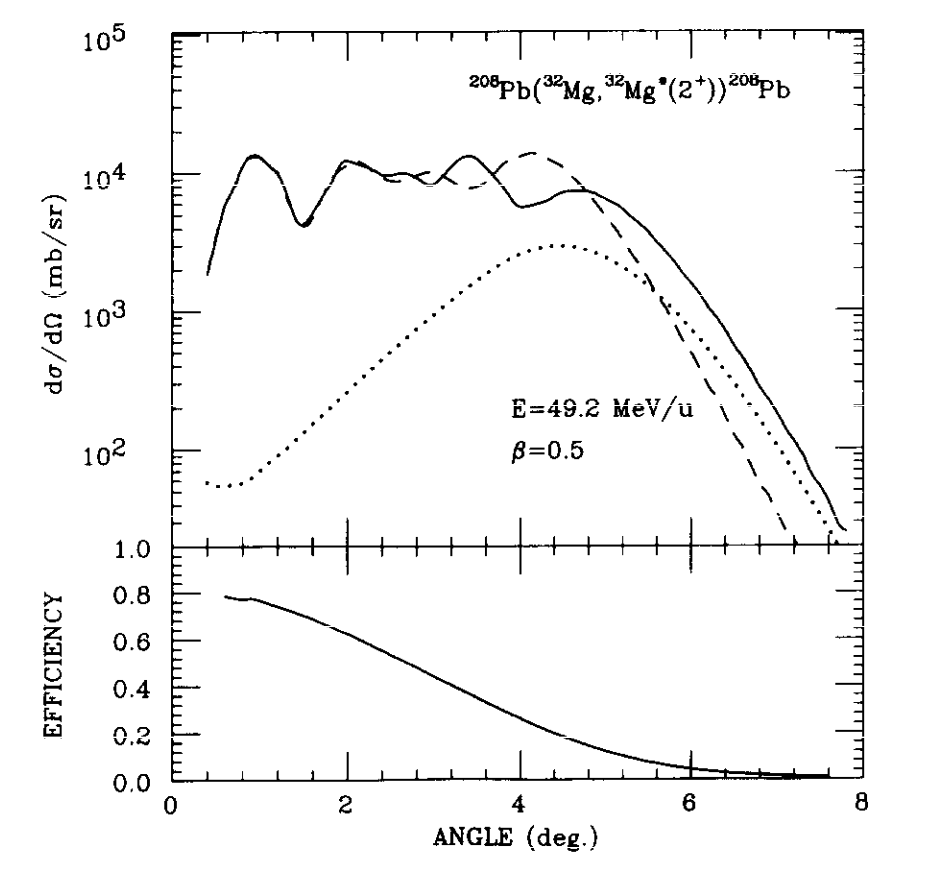
\includegraphics[trim={0 0 0 0.0cm},clip,width=0.95\textwidth]{images/motobayashi2}
            \\ \small{\cite{Motobayashi:1995ei}}
          \end{center}
        \end{block}
      \end{column}
    \end{columns}

  \end{frame}

  \begin{frame}
    \frametitle{Measured Value of $B(E2)$ \\ \small{\textit{Motobayashi et al.}}}

    \begin{center}
      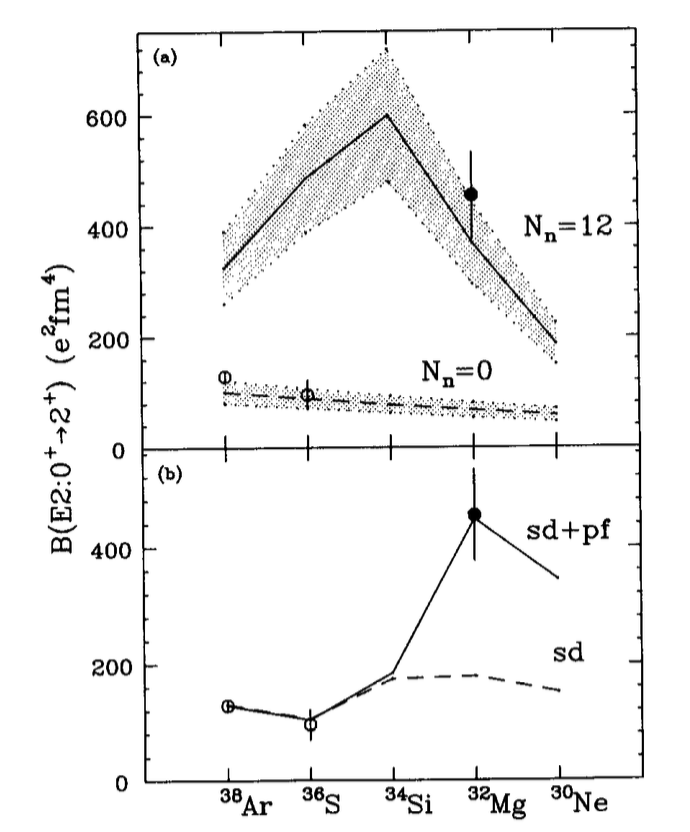
\includegraphics[trim={0 0 0 0.0cm},clip,width=0.38\textwidth]{images/motobayashi3}
      \\ \small{\cite{Motobayashi:1995ei}}
    \end{center}
  \end{frame}

\section{Appearance of the $N=16$ Shell Closure}

  \begin{frame}
    \frametitle{Observable: $S_n$ \\ \small{\textit{Ozawa et al.}}}
    \vskip-1em
    \begin{columns}[c]
      \begin{column}{0.5\textwidth}
        \begin{block}{}
          \begin{itemize}
            \item Neutron separation energy
            \item Determined by nucleus mass
          \end{itemize}
          \begin{equation*}
            S_n(^{40}Ca) = M(^{39}Ca) + M(n) - M(^{40}Ca)
          \end{equation*}
          \vskip-0.8em
          \begin{itemize}
            \item Mass measured by Penning traps and time-of-flight methods
            \item Penning traps:
            \begin{itemize}
              \item Required intensity: \textasciitilde10 pps
              \item Precision: \textasciitilde1 keV
            \end{itemize}
            \item Time-of-flight:
            \begin{itemize}
              \item Required intensity: \textasciitilde0.1 pps
              \item Precision: \textasciitilde100 keV
            \end{itemize}
          \end{itemize}
        \end{block}
      \end{column}
      \begin{column}{0.5\textwidth}
        \begin{center}
          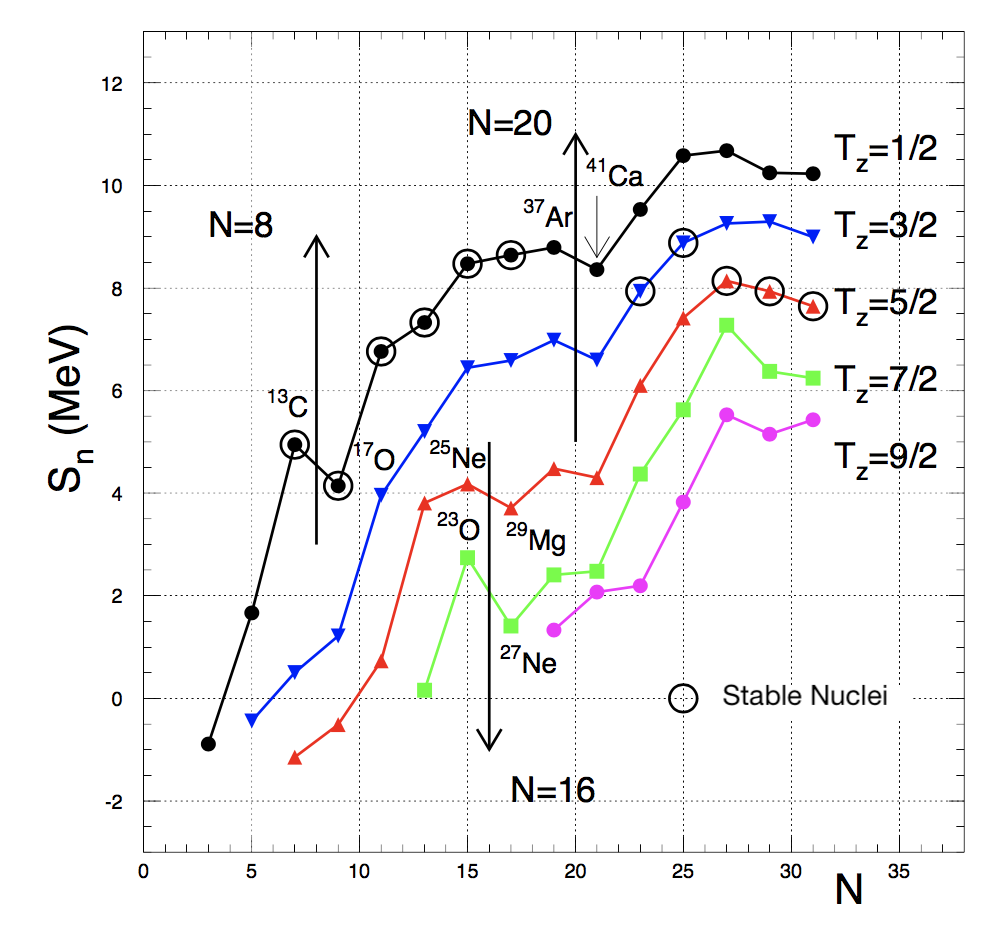
\includegraphics[width=0.95\textwidth]{images/ozawa_modified}
          \\ \small{Data:~\cite{Ozawa:2000gj}}
          \\ \small{Base figure:~\cite{Obertelli:2018personal}}
        \end{center}
      \end{column}
    \end{columns}
  \end{frame}

  \begin{frame}
    \frametitle{Observable: $E_x(2^+)$}
    \begin{itemize}
      \item Excitation energy to $J^P=2^+$ state
      \item First excited state is $2^+$ in almost all even-even nuclei
      \item Near stability, measured via $\beta$-decay
      \item For exotic nuclei, measured via in-beam gamma spectroscopy
      \begin{itemize}
        \item Required intensity: \textasciitilde10 pps
        \item Precision: \textasciitilde1--10 keV
      \end{itemize}
    \end{itemize}
  \end{frame}

  \begin{frame}
    \frametitle{Measuring $E_x(2^+)$ of $^{24}O$ \\ \small{\textit{Tshoo et al.}}}
    \vskip-2em
    \begin{columns}[c]
      \begin{column}{0.5\textwidth}
        \begin{block}{}
          \begin{itemize}
            \item Proton inelastic scattering
            \item $^{24}O{(p, p')}^{24}O* \rightarrow\ ^{23}O + n$
            \item Excited states are unbound
            \item Measure $^{23}O$ and $n$ invariant mass
            \item Determine decay energy
            \begin{itemize}
              \item $E_{decay}=0.56\pm0.05$ MeV
            \end{itemize}
            \item Compute excitation energy
            \item Need to know $S_n$
            \begin{itemize}
              \item $S_n=4.09\pm0.13$ MeV
            \end{itemize}
            \item $E_x(2^+)=4.65\pm0.14$ MeV
          \end{itemize}
        \end{block}
      \end{column}
      \begin{column}{0.5\textwidth}
        \begin{block}{}
          \begin{center}
            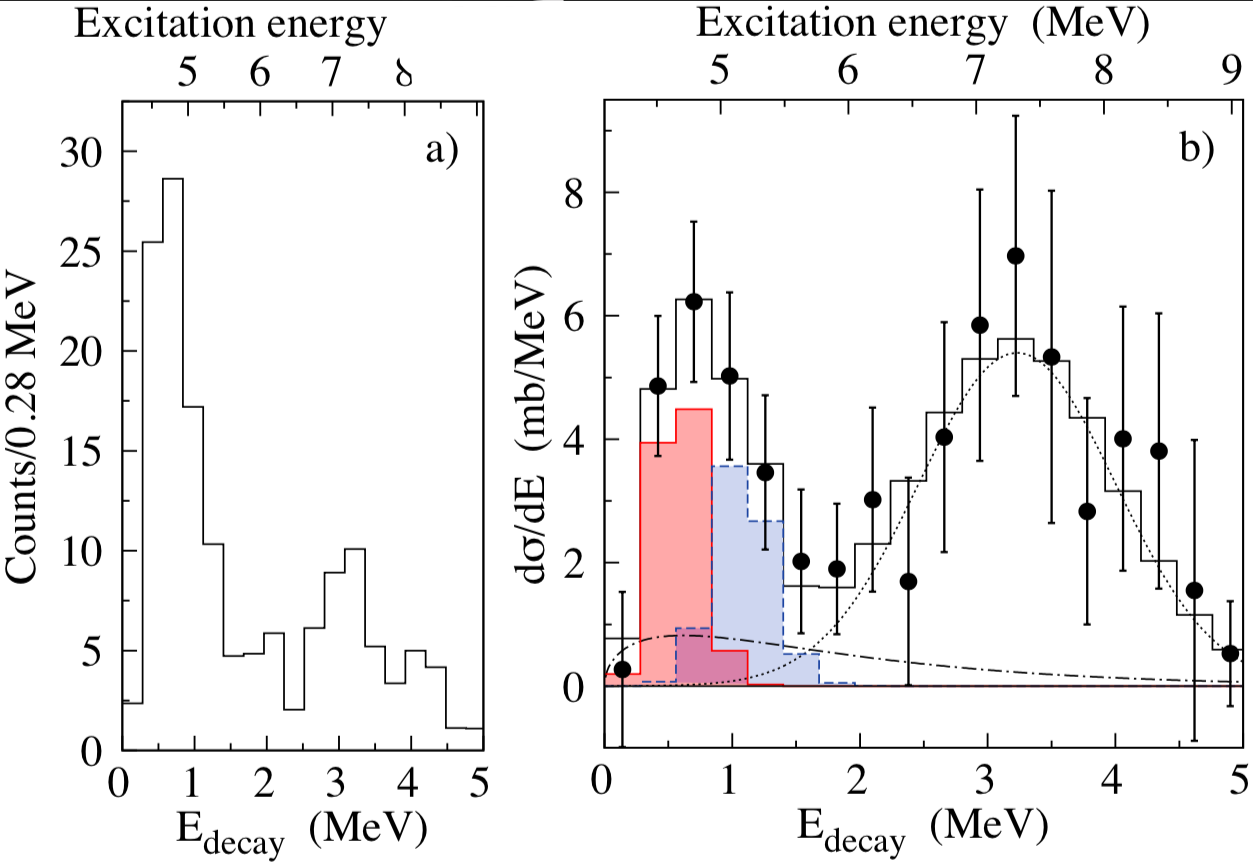
\includegraphics[trim={18.0cm 0 0 0.2cm},clip,width=0.7\textwidth]{images/tshoo2}
            \\ \small{\cite{Tshoo:2012bi}}
          \end{center}
        \end{block}
      \end{column}
    \end{columns}
  \end{frame}

  \begin{frame}
    \frametitle{Measuring $E_x(2^+)$ of $^{24}O$ \\ \small{\textit{Tshoo et al.}}}
    \begin{center}
      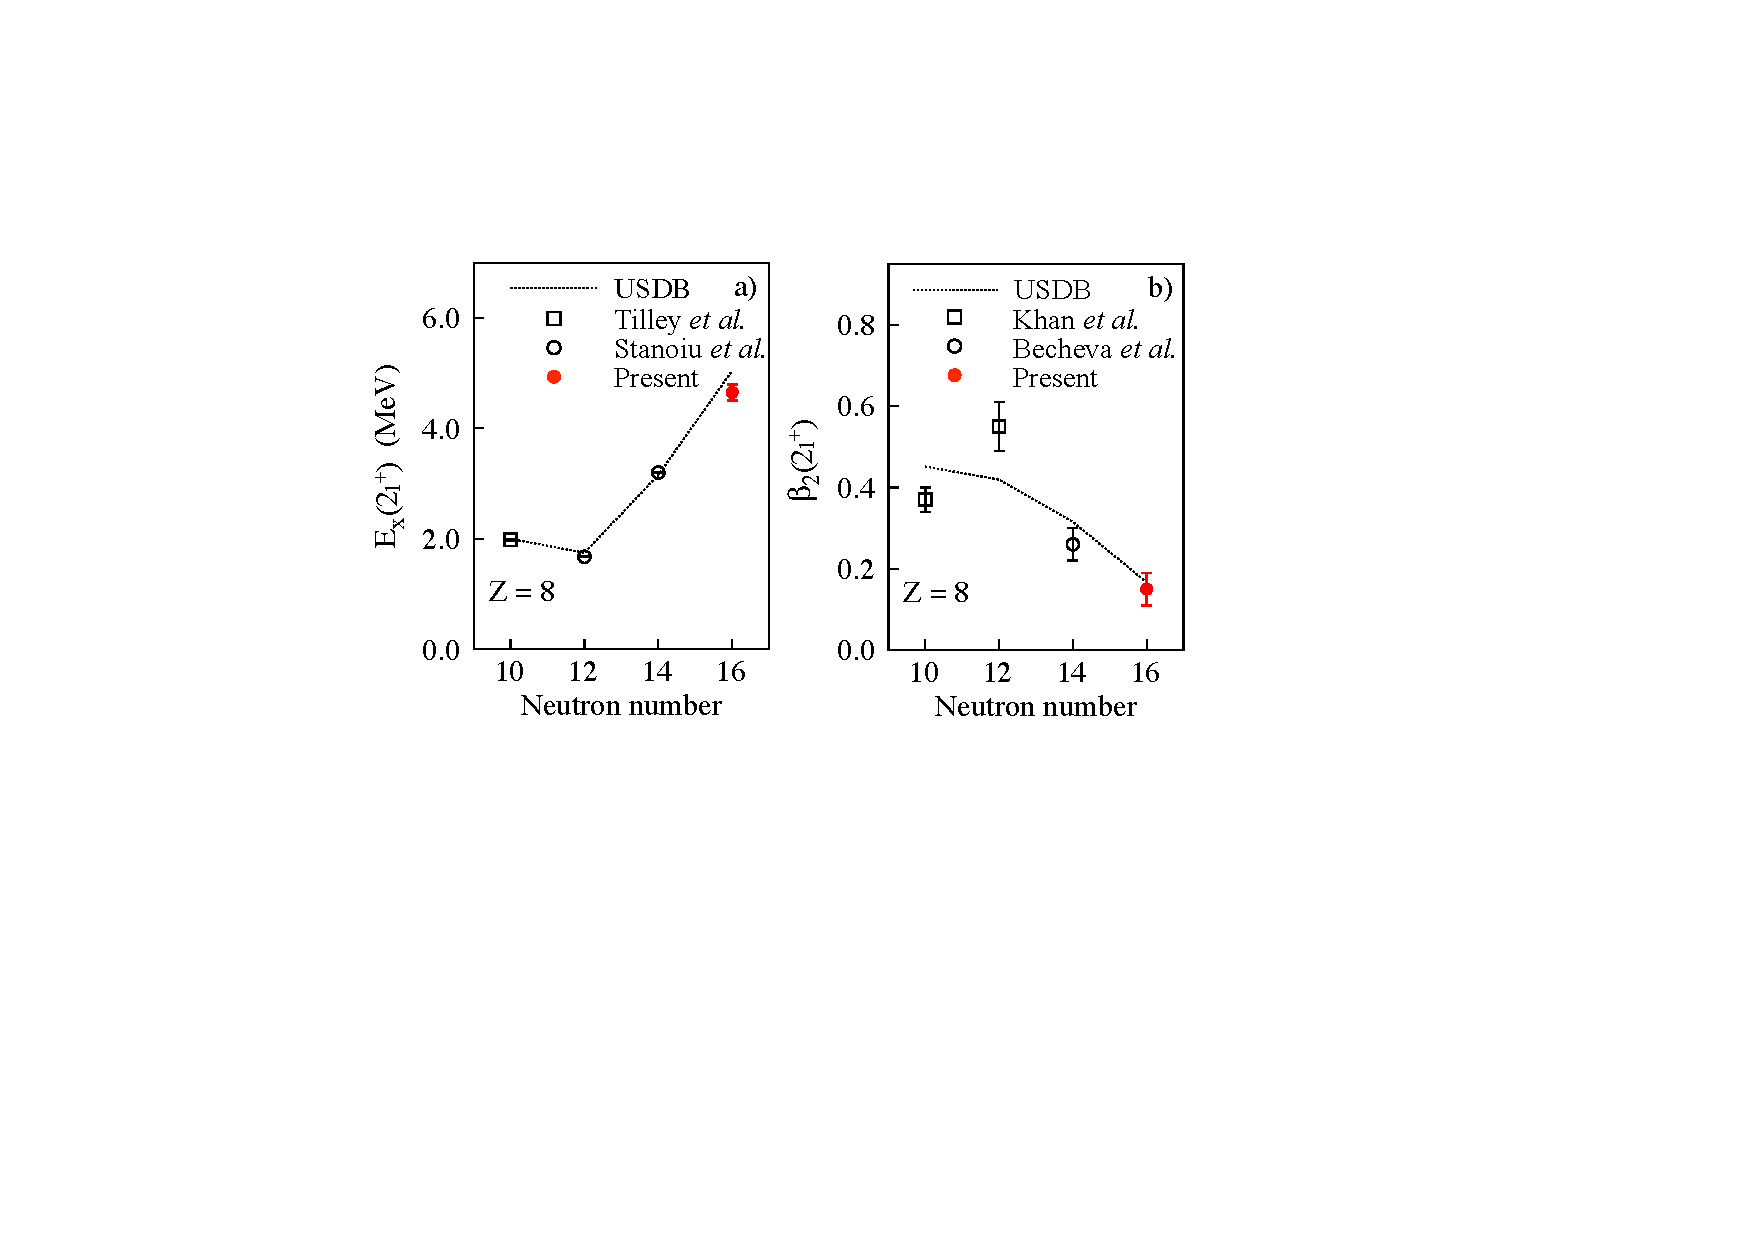
\includegraphics[trim={0 0 7cm 0},clip,width=0.41\textwidth]{images/tshoo4}
      \\ \small{\cite{Tshoo:2012bi}}
    \end{center}
  \end{frame}

  \begin{frame}
    \frametitle{$N=20$ and $N=16$ Recap}
    \begin{center}
      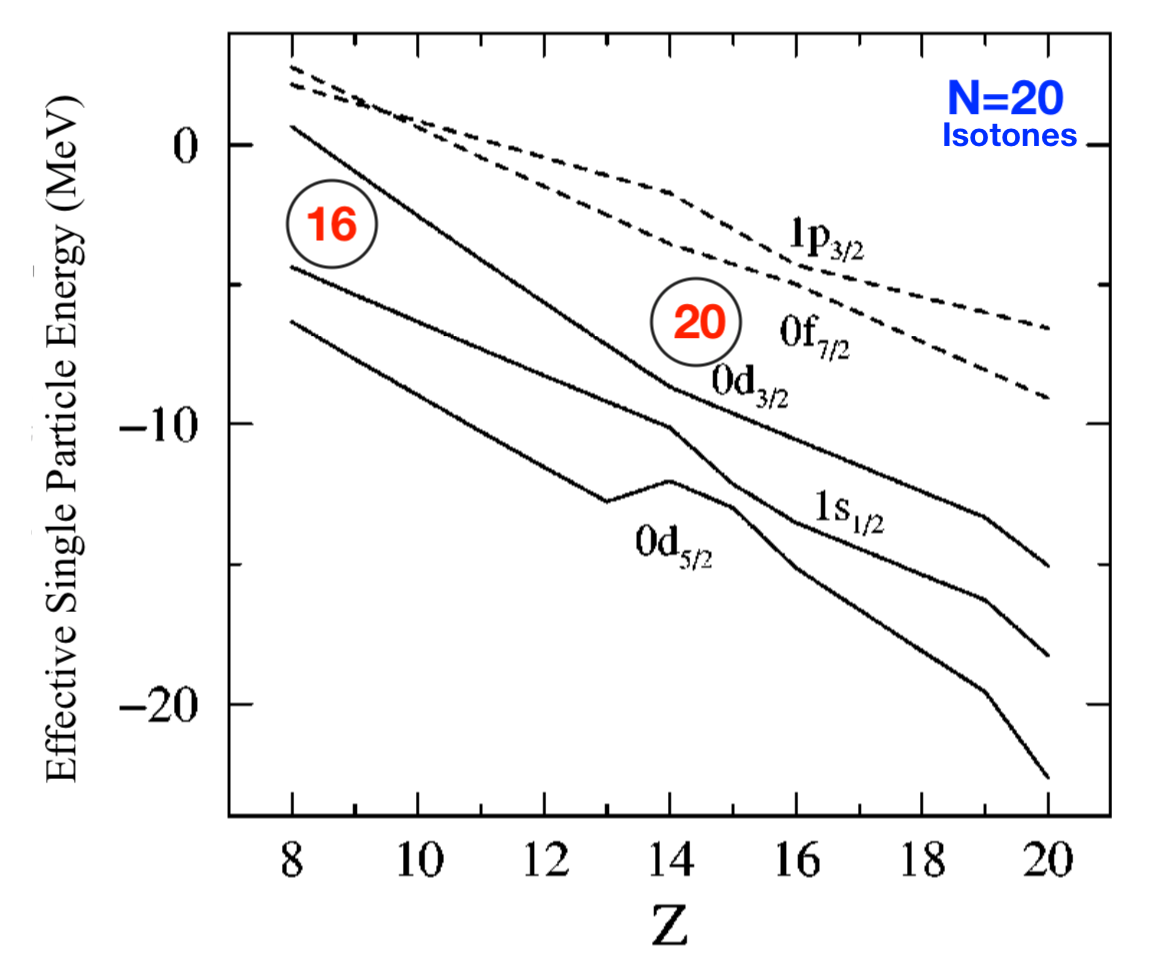
\includegraphics[trim={1.4cm 0 0 0},clip,width=0.55\textwidth]{images/utsuno_edited}
      \\ \small{\cite{Utsuno:1999st}}
    \end{center}
  \end{frame}

\section{Modern Frontiers for Shell Evolution}

  \begin{frame}
    \frametitle{Modern Frontiers for Shell Evolution}
    \begin{itemize}
      \item Are $N=32$ and $N=34$ ``magic numbers'' for $Ca$?
      \item What are the properties of $^{78}Ni$ and $^{100}Sn$?
      \item What are shell closures for super heavy elements?
    \end{itemize}
    \begin{center}
      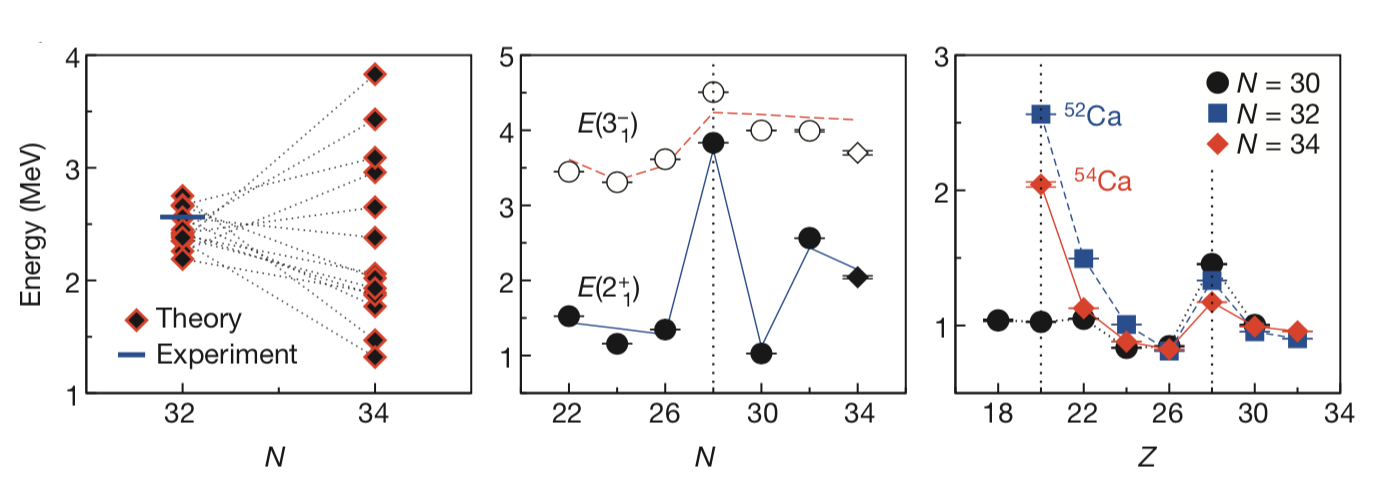
\includegraphics[trim={0 0 46.5cm 0},clip,height=0.35\textwidth]{images/steppenbeck2}
      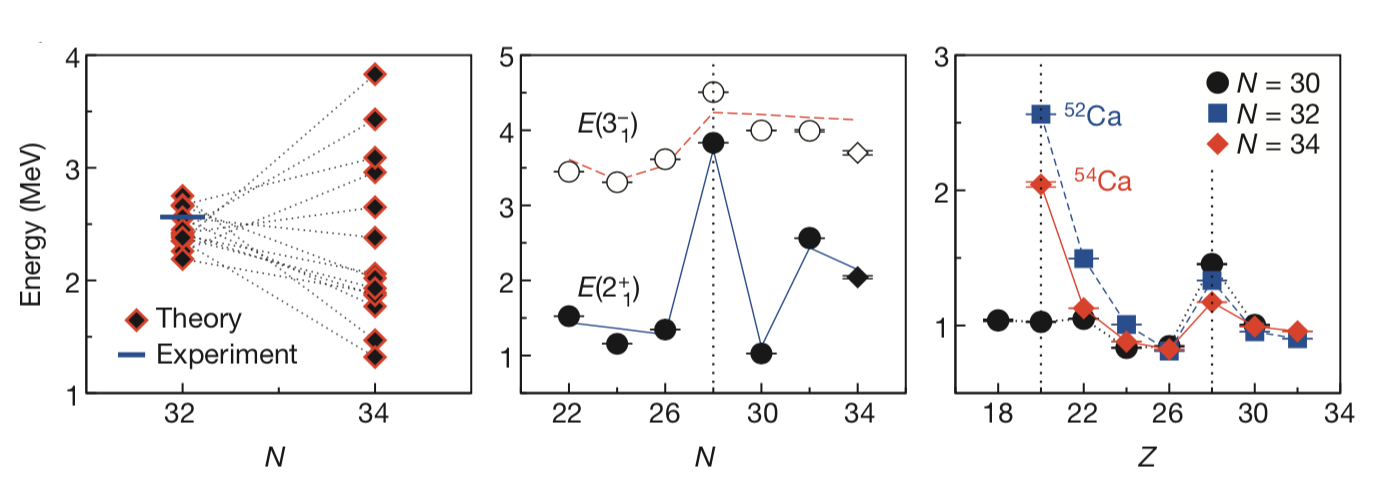
\includegraphics[trim={17cm 0 16cm 0},clip,height=0.35\textwidth]{images/steppenbeck2}
      \\ \small{\cite{Steppenbeck:2013mga}}
    \end{center}
  \end{frame}

\section{Summary}

  \begin{frame}
    \frametitle{Summary}
    \begin{itemize}
      \item Shells evolve and shell closures are not universal across the nuclear landscape
      \item Observable signs of shell closure:
      \begin{itemize}
        \item Low $B(E2)$
        \item Large binding energy
        \item High $E(2^+)$
        \item Small $r_{rms}$
        \item Long lifetime
      \end{itemize}
    \item Still many unexplored regions
    \item New facilities currently being constructed to explore these effects
    \end{itemize}
  \end{frame}

  \begin{frame}[allowframebreaks]
    \frametitle{References}
    \bibliographystyle{apalike}
    \bibliography{bibfile}
  \end{frame}

\end{document}
